\subsection{HTTP request}
Calling webservices uses HTTP protocols. 

To execute this, \textbf{a separate thread is necessary} as well as a manifest permission:

\begin{lstlisting}
<uses-permission android:name="android.permission.INTERNET"/>
\end{lstlisting}

After API 27, only HTTPS is allowed by default. Use \texttt{android:usesCleartextTraffic="true"}  in the 
\texttt{<}application\texttt{>} manifest tag for allowing HTTP. 

\begin{lstlisting}[title=Using HttpURLConnection]
private class AddUser(val address: String, val uname: String) : Runnable {
    override run() {
        val url: URL? = null
        val urlConnection: HttpURLConnection? = null
        try {
        // Configure -------------------------------------------
        url = URL("http://" + address + ":8701/Rest/users")
        urlConnection = url.openConnection() as HttpURLConnection
        urlConnection!!.setDoOutput(true)
        urlConnection!!.setDoInput(true)
        urlConnection!!.setRequestMethod("POST")
        urlConnection.!!setRequestProperty("Content-Type", "application/json")
        urlConnection!!.setUseCaches(false)

        // Payload ---------------------------------------------
        val outputStream = DataOutputStream(urlConnection!!.getOutputStream())
        val payload = "\"" + uname + "\""
        outputStream.writeBytes(payload)
        outputStream.flush()
        outputStream.close()

        // Response --------------------------------------------
        val responseCode = urlConnection!!.getResponseCode()
        if (responseCode == 200)
        val response = readStream(urlConnection!!.getInputStream(); // ... and transmit to UI
        }
        catch (Exception e) { . . . // treat the exception
        }
        finally {
            if(urlConnection != null) urlConnection.disconnect()
        }
    }
}
\end{lstlisting}

\begin{lstlisting}[title=Using threads to invoke]
val addUser = AddUser(address, name)
val thr = Thread(addUser)
thr.start();
\end{lstlisting}

\subsection{Threads}
When an application is launched, the system creates a thread of execution for the 
application, called "main." This thread is in charge of dispatching events to the 
appropriate user interface widgets and for interacting with components from the Android UI 
toolkit. As such, the main thread is also sometimes called the UI thread. 


Android UI toolkit is not thread-safe. So, you must not manipulate your UI from a 
worker thread—you must do all manipulation to your user interface from the UI thread. 
Activity.runOnUiThread(Runnable) is a way to access the UI thread from another thread to 
solve this problem.

\subsection{Communication between threads}
The problem with the java communication systems between threads (e.g pipes, blocking queue, 
shared memory, etc) is that these mechanisms are blocking. Since the communication between threads
are mainly done between the UI thread and background threads, an android mechanism was created to handle
this communication. 

\subsubsection{Handlers}

\begin{figure}[h]
\centering
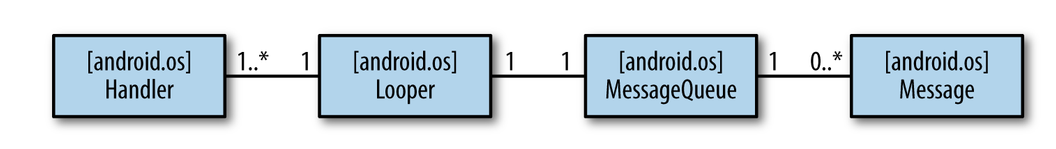
\includegraphics[width=0.8\linewidth]{figures/05_thread_handler_overview.png}
\caption{Thread handler overview}
\label{fig:thread_handler_overview}
\end{figure}

\begin{itemize}
    \item \texttt{android.os.Looper}: A message dispacher associated with one and only 
    one cosumer thread. 
    \item \texttt{android.os.Handler}: Consumer thread message processor, and 
    the interface for a producer thread to insert messages into the queue.
    A Looper can have many associated handlers, but they \textbf{all insert messages into 
    the same queue}.
    \item \texttt{android.os.MessageQueue}: Unbounded linked list of messages to be processed 
    on the consumer thread. Every Looper - and Thread - has at most one MessageQueue.
    \item \texttt{android.os.Message}: Message to be executed on the consumer thread.
\end{itemize}



\begin{lstlisting}[title=Send messages between threads]
// Cosumer threads 
MyHandler(val uiActivity: MyActivity) { 
    override handleMessage(m: Message) { 
        val s = m.getData().getString("msgstr") 
        // ... uiActivity.doSomething(s) 
    } 
}

// Producer threads
MyRunnable(val uiHandler: Handler) { 
    fun run() { 
        ...interact()...
    } 
    fun interact() { 
        val m = uiHandler.obtainMessage() 
        m.setData(createBundleFromStr("something")) 
        // boolean sendMessage(Message msg)
        uiHandler.sendMessage(m) // Send message to the queue. 
    } 
}
    
// In the activity
val myHandler = MyHandler(this)
val worker = Thread(MyRunnable(myHandler))
worker.start()
    
\end{lstlisting}

The code above follows the schema:
\begin{figure}[h]
\centering
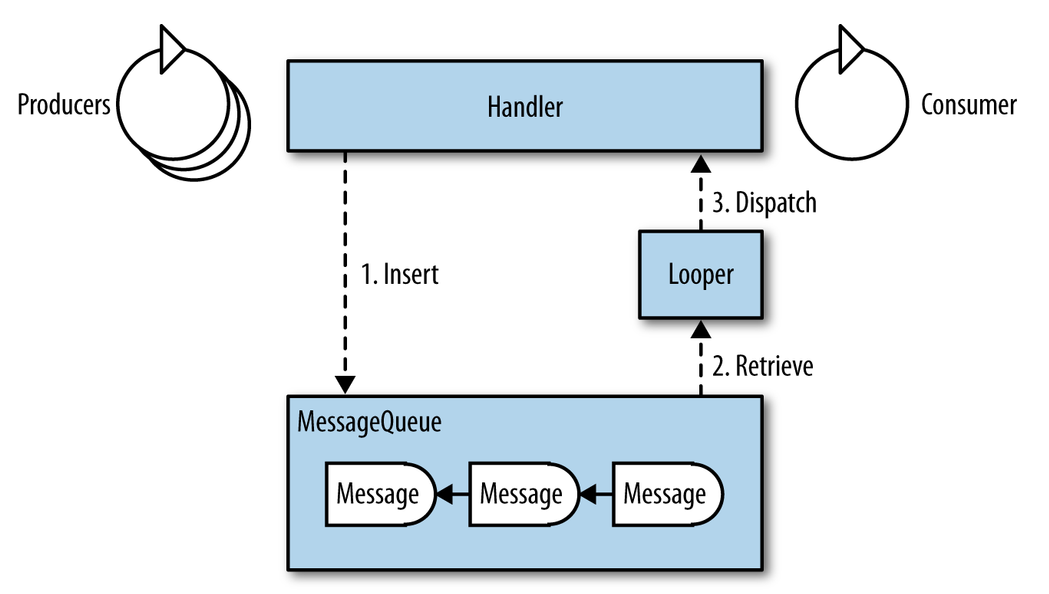
\includegraphics[width=0.8\linewidth]{figures/05_handler_schema.png}
\caption{Sending message flow schema}
\label{fig:handler_schema}
\end{figure}


\newpage
\subsubsection{Messages as Tasks (Post)}
The Handler inserts messages in the message queue in various ways depending on the 
message type. 
\begin{itemize}
    \item Task messages are inserted through methods that are prefixed post;
    \item Data insertion methods are prefixed send, like we saw in the previous section. 
\end{itemize}

To add a task in a queue we can do:
\begin{lstlisting}
boolean post(Runnable r)
\end{lstlisting}


\begin{lstlisting}[title=Post an no parameters]
private val handler = Handler()

private fun mainProcessing() { 
    val thread = Thread(doBackgroundThreadProcessing, "Background") 
    thread.start() 
} 
    
private val doBackgroundThreadProcessing = Runnable() {
    override run() { 
        [ ... Time consuming operations ... ]
        handler.post(doUpdateGUI) // send a task to the queue. 
    } 
}
    
// Runnable that updates GUI on the UI thread
val doUpdateGUI = Runnable() { 
    override run() { 
        [ ... Open a dialog or modify a GUI element ... ] 
    } 
};

\end{lstlisting}
\newpage
\subsection{Async Task}
The message passing mechanism between thread is a \textbf{nonblocking} consumer-producer pattern. 
\begin{lstlisting}[title=Creating and running Async tasks]
// AsyncTask<[Input Parameter Type], [Progress Report Type], [Result Type]>
private class MyAsyncTask() : AsyncTask<String, Int, Int> {
    // Is also executed by the UI thread when the background task call publishProgress.
    There is parameter passing between these methods. 
    override onProgressUpdate(progress: Int) {
        // [... Update progress bar, Notification, or another UI element ...]
    }

    // Is executed by the UI Thread when doInBackground finishes. 
    override onPostExecute(result: Int) {
        // [... Report results via UI update, Dialog, or notification ...]
    }

    // Is executed by a background task when AsyncTask is excuted.
    override doInBackground(parameter: String ): Int {
        val myProgress = 0
        // [... Perform background processing task, update myProgress...]
        publishProgress(myProgress)
        // [... Continue performing background processing task ...]
        // Return the value to be passed to onPostExecute
        return result
    }
}

// Executing 
MyAsyncTask().execute("inputString");
    
\end{lstlisting}











